\chapter{Direct Methods of Proof}
\begchap{N}ow that we have learned the basic mechanisms of proof, we will focus our attention to actually using these mechanisms to prove things. The following chapter introduces you to various types of proofs, beginning with the most common types and moving to the least common, walking through common traps. It is very important to understand these concepts and thus I highly recommend you follow this chapter with diligence, and try to attempt the exercises and problems. This chapter, and perhaps most chapters beyond this point, require significantly more resilience and ingenuity than is typical in school or early college; to follow through, and so, do not be discouraged! Do not be afraid to ask questions as they arise (many answers can also be found online), and/or try your own variations on the themes presented. Proofs are an art; mathematics is our brushstrokes. While painters may be praised for their creativity, all painters must learn the mechanisms by which to paint on a canvas (or other medium); which is a skill that can only be developed through much practice!





\section{Basic Direct Proof}
We will introduce proofs through a basic example, which we will prove subsequently, walking through the steps of a direct proof.
\begin{example}
The sum of two odd integers is even.
\end{example}
We can first identify the formal if then statement from the above. We will also convert this into math notation. While such a step is not strictly needed, math notation is used for a reason!
\[
\forall a,b\in \mathbb{Z} ~\text{~such that ~}~ 2 \nmid a ~\text{~ and ~}~ 2 \nmid b \implies 2\mid a+b
\]
Where the $p\mid q$ denotes that $p$ divides $q$ (there is no remainder; this statement is equivalent to saying there exists some integer $k$ where $pk = q$), and $p \nmid q$ indicates that $p$ does not divide $q$. 

We will prove this via direct proof.

\begin{proof}
Every odd number $n$ can be written as $2k+1$ for some $k \in \mathbb{Z}$. Thus, $\exists \alpha, \beta \in \mathbb{Z}$ such that $a = 2\alpha + 1$ and $b = 2\beta + 1$. Note that we have that $2 \nmid a,b$ since they will always leave remainder 1. Their sum is then 
\[
a + b = 2\alpha + 2\beta + 2
\]
which is evidently divisible by 2 with quotient $\alpha + \beta + 1$ and no remainder. $ 2 \mid a + b$. Thus, the sum of two odd integers $a$ and $b$ is even.
\end{proof}

Although that was a relatively short proof, it demonstrates a simple example of a direct proof. Note that we have had to make many assumptions in order to prove this. Most of these assumptions are assumptions about the functions of numbers, but we will not prove these (we won't prove that 2 is a number, etc.) in that they are trivial\footnote{Meaning exceptionally easy or obvious.}; should you be constructing your own proof such things will also not need proof. However, an important claim we have made without proving is that every odd number $n$ may be written as $2k+1$ for some integer $k$. This is again a very simple example and in this case it may be stated without proof. However, oftentimes such intermediate statements that we assume to be true may need to be proven individually. We can call this smaller, supporting statements lemmas, which support in proving a theorem.

Further note the direct nature of this proof; we use methods to directly show that the original assumptions $P$ directly imply that the statement $Q$ is true, which proves $P \implies Q$. 

Consider the diagram below. We will aim to prove the following statement, known as the inscribed angle theorem.

\begin{center}
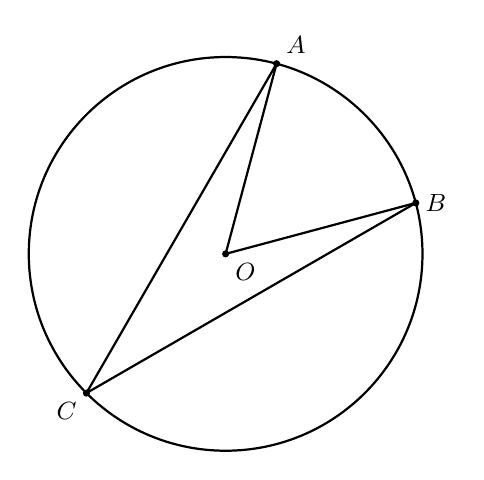
\begin{tikzpicture}[scale=2.5]

  % Circle
  \draw[thick] (0,0) circle (1);
  
  % Center
  \filldraw[black] (0,0) circle (0.015) node[below right, font=\small] {$O$};

  % Points A and B near each other (upper right area)
  \coordinate (A) at (75:1);
  \coordinate (B) at (15:1);
  
  % Point C opposite (lower left area)
  \coordinate (C) at (225:1);

  % Draw points
  \filldraw[black] (A) circle (0.015) node[above right, font=\small] {$A$};
  \filldraw[black] (B) circle (0.015) node[right, font=\small] {$B$};
  \filldraw[black] (C) circle (0.015) node[below left, font=\small] {$C$};

  % Lines CA and CB
  \draw[thick] (C) -- (A);
  \draw[thick] (C) -- (B);

  % Lines OA and OB (radii)
  \draw[thick] (0,0) -- (A);
  \draw[thick] (0,0) -- (B);

\end{tikzpicture}
\end{center}

\begin{theorem} [Inscribed Angle Theorem]
Consider the diagram below. Prove that $\angle AOB = 2 \angle ACB$.
\end{theorem}

The following proof will use some basic facts about circles and isosceles triangles. In the most formal setting possible, it would be necessary to present proofs of these smaller facts. However, in nearly every case (I can't think of a case where you \emph{would} need to present a proof of these basic facts) it is better to present such basic facts without a proof. We will discuss more about the formality and thoroughness of proofs towards the end of this chapter. For now, just pay attention to how direct proof is used in geometry. 

\begin{proof}
Since $O$ is the center of the circle, each segment $OA, OB, OC$ is a radius of the circle, and thus they have the same length: 
\[
\overline{OA} = \overline{OB} = \overline{OC}
\]
Since $\overline{OA} = \overline{OC}$, $\triangle AOC$ is isosceles. Similarly, since $\overline{OA} = \overline{OB}$, $\triangle AOB$ is isosceles. This is shown in the diagram below. 

\begin{center}
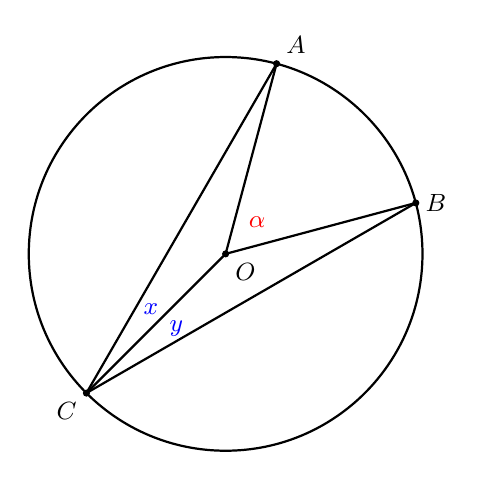
\begin{tikzpicture}[scale=2.5]

  % Circle
  \draw[thick] (0,0) circle (1);
  
  % Center
  \filldraw[black] (0,0) circle (0.015) node[below right, font=\small] {$O$};

  % Points A and B near each other (upper right area)
  \coordinate (A) at (75:1);
  \coordinate (B) at (15:1);
  
  % Point C opposite (lower left area)
  \coordinate (C) at (225:1);

  % Draw points
  \filldraw[black] (A) circle (0.015) node[above right, font=\small] {$A$};
  \filldraw[black] (B) circle (0.015) node[right, font=\small] {$B$};
  \filldraw[black] (C) circle (0.015) node[below left, font=\small] {$C$};

  % Lines CA and CB
  \draw[thick] (C) -- (A);
  \draw[thick] (C) -- (B);

  % Lines OA and OB (radii)
  \draw[thick] (0,0) -- (A);
  \draw[thick] (0,0) -- (B);

  % Line OC (extended to circle, drawn dashed)
  \draw[thick] (0,0) -- (C);

  % Angle x at C between CA and OC (left part of inscribed angle)
  \node[blue, font=\small] at (-0.38, -0.28) {$x$};

  % Angle y at C between OC and CB (right part of inscribed angle)
  \node[blue, font=\small] at (-0.25, -0.38) {$y$};

  % Angle alpha at O (central angle)
  \node[red, font=\small] at (0.16, 0.16) {$\alpha$};

\end{tikzpicture}
\end{center}

Notice that $\angle ACB$ is split into $\angle ACO$ and $\angle OCB$, which we have labeled $x$ and $y$, respectively. Note that since $\triangle AOB$ is isosceles, the two base angles must be equal. Since $\overline{OC} = \overline{OA}$, we have the following relationship
\[
\angle OCA = \angle OAC = x
\]
Further, the angles of all triangles must sum to $180^{\circ}$. Using this, we can calculate the measure of angle $\angle AOC$. 
\[
\angle OCA + \angle OAC + \angle AOC = 180^{\circ}
\]
\[
2x + \angle AOC = 180^{\circ}
\]
\[
\angle AOC = 180^{\circ} - 2x
\]
Similarly, we use the same argument for $\triangle BCO$ to obtain
\[
\angle OCB = \angle OBC = y
\]
and therefore
\[
\angle OCB + \angle OBC + \angle BOC = 180^{\circ}
\]
\[
2y + \angle BOC = 180^{\circ}
\]
\[
\angle BOC = 180^{\circ} - 2y
\]
The new angles are shown in the figure below.
\begin{center}
\begin{tikzpicture}[scale=2.5]
  % Circle
  \draw[thick] (0,0) circle (1);
  
  % Center
  \filldraw[black] (0,0) circle (0.015);

  % Points A and B near each other (upper right area)
  \coordinate (A) at (75:1);
  \coordinate (B) at (15:1);
  
  % Point C opposite (lower left area)
  \coordinate (C) at (225:1);

  % Draw points
  \filldraw[black] (A) circle (0.015) node[above right, font=\small] {$A$};
  \filldraw[black] (B) circle (0.015) node[right, font=\small] {$B$};
  \filldraw[black] (C) circle (0.015) node[below left, font=\small] {$C$};

  % Lines CA and CB
  \draw[thick] (C) -- (A);
  \draw[thick] (C) -- (B);

  % Lines OA and OB (radii)
  \draw[thick] (0,0) -- (A);
  \draw[thick] (0,0) -- (B);

  \draw[thick] (0,0) -- (C);

  % Angle x at C left (between CA and OC)
  \node[blue, font=\small] at (-0.38, -0.28) {$x$};

  % Angle y at C right (between OC and CB)
  \node[blue, font=\small] at (-0.25, -0.38) {$y$};

  % Angle x at A (base angle of isosceles triangle OAC)
  \node[blue, font=\small] at ($(A) + (-0.17, -0.4)$) {$x$};

  % Angle y at B (base angle of isosceles triangle OBC)
  \node[blue, font=\small] at ($(B) + (-0.45, -0.19)$) {$y$};

  % 180 - 2x at O for triangle OAC
  \node[red, font=\scriptsize] at (-0.23, 0.02) {$180^{\circ}\!-\!2x$};

  % 180 - 2y at O for triangle OBC
  \node[red, font=\scriptsize] at (0.18, -0.12) {$180^{\circ}\!-\!2y$};

  % Alpha at O (central angle AOB)
  \node[red, font=\small] at (0.16, 0.16) {$\alpha$};

\end{tikzpicture}
\end{center}
Finally, we know that the angles at the center of the circle must add to $360^{\circ}$. Therefore,
\[
\angle AOB + \angle BOC + \angle COA = 360^{\circ}
\]
\[
\alpha + 180^{\circ} - 2y + 180^{\circ} - 2x = 360^{\circ}
\]
\[
\alpha = 2x + 2y = 2(x+y)
\]
and since $\angle ACB = \angle ACO + \angle OCB = x + y$ and $\angle AOB = \alpha$, we get
\[
\angle AOB = 2 \angle OCB
\]
Which proves the inscribed angle theorem. 
\end{proof}

For some background information, $\angle ACB$ is called the inscribed angle in this scenario, while $\angle AOB$ is typically called the central angle. This theorem applies to all pairs of inscribed and central angles and is a central result in geometry, one you will use at some point in your lifetime, even if you do not plan to pursue math. The theorem, in its most general form, shows that the measure of the central angle is twice the measure of the inscribed angle, given that both angles subtend the same arc (arc $\overset{\frown}{AB}$ in this case). Remember this theorem, you will use it often!

\begin{theorem}[Inscribed Angle Theorem]
For points $A, B, C$ on a circle with center $O$, $\angle AOB = 2 \angle ACB$.
\begin{center}
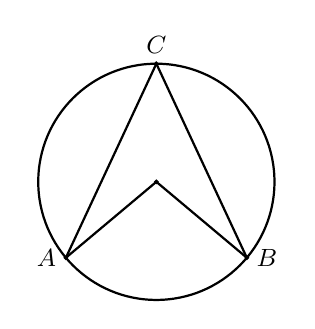
\begin{tikzpicture}[scale=1.5]
  % Circle
  \draw[thick] (0,0) circle (1);
  
  % Center
  \filldraw[black] (0,0) circle (0.015);

  % Points A and B near each other (upper right area)
  \coordinate (A) at (220:1);
  \coordinate (B) at (320:1);
  
  % Point C opposite (lower left area)
  \coordinate (C) at (90:1);

  % Draw points
  \filldraw[black] (A) circle (0.015) node[left, font=\small] {$A$};
  \filldraw[black] (B) circle (0.015) node[right, font=\small] {$B$};
  \filldraw[black] (C) circle (0.015) node[above, font=\small] {$C$};

  % Lines CA and CB
  \draw[thick] (C) -- (A);
  \draw[thick] (C) -- (B);

  % Lines OA and OB (radii)
  \draw[thick] (0,0) -- (A);
  \draw[thick] (0,0) -- (B);

\end{tikzpicture}
\end{center}
\end{theorem}

This example demonstrated direct proof in geometry. Proofs are not limited to algebraic manipulation or number theory. Direct proof, especially, is the most widely used method of proof and is ubiquitous across mathematical domains. In this specific example, we used a geometric technique called angle chasing, as we simply assigned variables to angles and solved for all other angles, until we got an equation through which we could relate the inscribed and central angles. We derived an equation relating the two angles, and solved to get the relationship between them. 

As a more general note, it is always useful to draw diagrams for geometry problems. Don't be afraid to draw them big or multiple times, I have ended up using four diagrams to explain the proof of the theorem and the general form of the theorem. Diagrams make it easy to visualize the figure (how would you do the proof while imagining the figure in your head?) and generate new ideas (such as the isosceles triangle idea). Always draw diagrams/figures!

We will now move on to a more difficult example of direct proof in algebra. The following is a useful identity for polynomial functions of the following form.

\begin{example}
Prove that for all distinct integers $a$ and $b$, 
\[a^k-b^k = (a-b)(a^{k-1} + a^{k-2}b + \cdots + b^{k-1})\]
\end{example}
\begin{proof}
We will show that the right-hand-side (RHS) equals the left-hand-side (LHS) in the above equation.
\[
(a-b)(a^{k-1} + a^{k-2}b + \cdots + b^{k-1}) = (a-b)\left(\sum_{i=1}^{k}{a^{k-i}b^{i-1}}\right)
\]
By the distributive property, we get
\[
(a-b)\left(\sum_{i=1}^{k}{a^{k-i}b^{i-1}}\right) = a \left(\sum_{i=1}^{k}{a^{k-i}b^{i-1}}\right) - b\left(\sum_{i=1}^{k}{a^{k-i}b^{i-1}}\right)
\]
\[
= \sum_{i=1}^{k}{a^{k-i+1}b^{i-1}} - \sum_{i=1}^{k}{a^{k-i}b^{i}}
\]
\[
= (a^{k} + a^{k-1}b + \cdots + a^2b^{k-2} + ab^{k-1} ) 
\]
\[
- (a^{k-1}b + a^{k-2}b^2 + \cdots + ab^{k-1} + b^k)
\]
The middle terms cancel via addition, leaving only the first term of the first sum and the last term of the last sum, which results in 
\[
a^k - b^k
\]
which equals the LHS.
\[
\therefore ~~ a^k-b^k = (a-b)(a^{k-1} + a^{k-2}b + \cdots + b^{k-1})
\]
\end{proof}

This was perhaps the most "direct" proof possible, in which we simply multiply the terms and show that the identity holds. Note that, for the specific wording of this problem, we do not need to derive the identity mathematically, we just need to show that it holds true, and thus we can resort to short-cut type proofs as shown. A second remark is that of the use of the summation notation. It is standard in proofs to rely on the use of summation notation in order to index every term, as opposed to the final step we did where we used the long sums in equation (3.1) and argued that select terms are additive inverses of each other. While this approach by explicit listing with ellipses is not wrong, it is oftentimes helpful to get acquainted with summation notation for the value it provides, as here we assumed that the terms in the ellipses cancel each other out. It is a valid assumption in this context, since there is a clear pattern and we can clearly show that they do cancel. However, it is best to use summation notation for exactitude. We could thus replace that step (equation 3.1) with 
\[
= a^k + \sum_{i=2}^{k}a^{k-i+1}b^{i-1} - \left(  \sum_{i=1}^{k-1}{a^{k-i}b^{i}} + b^k \right)
\]
\[
= a^k - b^k + \sum_{i=2}^{k}a^{k-i+1}b^{i-1} - \sum_{i=1}^{k-1}{a^{k-i}b^{i}}
\]
in which we shift the index of the first summation down by 1 (let $j = i - 1$, $i = j+1$) to yield
\[
= a^k - b^k + \sum_{j=1}^{k-1}a^{k-(j+1)}b^{(j+1)-1} - \sum_{i=1}^{k-1}{a^{k-i}b^{i}}
\]
\[
=a^k - b^k
\]
in order to be more explicit. It oftentimes helps to do so, though in most cases, the argument with the ellipses would not get penalized since the behavior that is omitted by the ellipses is well defined (the prior sum notation), as opposed to some ill-defined ellipses such as 
\[\{1, 3, 7, 2, 5, 1, \ldots , 3242,4 3 \}\]
in which we have no clue as to what happens within the ellipses. If you are unfamiliar with summation notation or have not used it much, now is the time to get more familiar with it. It is your best friend for proofs such as these, as it makes expressions more explicit and stops us from getting caught up with "\ldots" - we know what is going on within. 

Consider the next example, a very useful result in number theory and basic algebra, and directly builds off of Example 3.1.2. With respect to this, it may be appropriate to denote Example 3.1.2 as a lemma if our primary intent was to prove the below theorem. While this theorem seems irrelevant or niche, it has a wide range of powerful applications, especially in olympiad problems.

\begin{example}
    Let $\mathbb{Z}[x]$ denote the set of polynomial functions with integer coefficients. For any two distinct integers $a$ and $b$, prove that $a - b  \mid P(a) - P(b)$ for all functions $P(x) \in \mathbb{Z}[x]$.
\end{example}

\begin{proof}
    Any polynomial $P(x)$ can be represented by a sum of the products of the coefficients and the variable raised to the respective power.
    \[
    P(x) = c_k \cdot x^k + c_{k-1} \cdot x^{k-1} + \cdots + a_1 \cdot c + a_0 = \sum_{i=0}^{k} c_ix^i 
    \]
    where $c_0, c_1, \ldots, c_k \in \mathbb{Z}$ are the coefficients of the function, and uniquely determine the specific polynomial $P(x)$. Then, for two distinct integers $a$ and $b$, we have 
    \[
    P(a) - P(b) = \sum_{i=0}^{k} c_ia^i -\sum_{i=0}^{k} c_ib^i  = \sum_{i=1}^{k}c_i(a^i-b^i) + c_0 - c_0
    \]
    \[
    =\sum_{i=1}^{k}c_i(a^i-b^i)
    \]
    Recall the factorization of differences of the form $(a^i -b^i)$ from Example 3.1.2.
    \[
    (a^i -b^i) = (a-b)(a^{i-1} + a^{i-2}b + \cdots + b^{i-1}) = (a-b)\left(\sum_{j=1}^{i}{a^{i-j}b^{j-1}}\right)
    \]
    Substitute this expression into the polynomial difference
    \[
    P(a) - P(b) = \sum_{i=1}^{k}c_i(a^i-b^i) = \sum_{i=1}^{k}\left(c_i(a-b)\left(\sum_{j=1}^{i}{a^{i-j}b^{j-1}}\right)\right) 
    \]
    \[
    = (a-b)\left(\sum_{i=1}^{k}\left(c_i\sum_{j=1}^{i}{a^{i-j}b^{j-1}}\right)\right)
    \]
    and thus $P(a) - P(b)$ will contain a factor of $(a-b)$. 
\end{proof}

This proof, instead of relying on "bashing" with multiplication as did Example 3.1.2, relied upon algebraic manipulation of quantities to derive a form in which $(a-b)$ is an explicit factor. Because we directly work with the original expression to derive a new form of the same expression in order to reason about divisibility, we still consider this to be direct proof. In fact, algebraic manipulation similar to this is a key technique in may problems involving equalities, expressions and/or inequalities that we must prove or derive properties about. Furthermore, this theorem is very important in many problem-solving contexts, and thus we will write a formal theorem statement for your reference. 

\begin{theorem}
     $\forall a, b \in \mathbb{Z}, a \neq b$,   \[a - b  \mid P(a) - P(b) ~~~ \forall P(x) \in \mathbb{Z}[x]\]
\end{theorem}

This theorem is quite widespread, and in most cases, can be stated, cited, and/or used without need to prove it. We do not need to "reinvent the wheel" in math olympiad cases or research cases. We will discuss this more in the note on thoroughness. 

We will now look at yet another highly useful theorem in olympiad algebra.
\begin{theorem}[Vieta's Formulas]
Given a polynomial $f$ of order $n$ with coefficients $a_n, a_{n-1}, \ldots, a_1, a_0 \in \mathbb{R}$ with roots $r_1, r_2, \ldots, r_n$ such that $f(r_i) = 0$ for all $1 \leq i \leq n$, Vieta's formulas are the following relations: 
\[
f(x) = \sum_{i=0}^{n} a_ix^i 
\]
\[
= a_nx^n + a_{n-1}x^{n-1} + \cdots + a_1x + a_0 = a_n(x-r_1)(x-r_2)\cdots(x-r_n)
\]
the following relations hold for its roots:
\[
\begin{cases}
r_1 + r_2 + \cdots + r_n = -\frac{a_{n-1}}{a_n} \\[1ex]
\begin{aligned}
&(r_1r_2 + r_1r_3 + \cdots + r_1r_n) \\
&\quad + (r_2r_3 + \cdots + r_2 r_n) + \cdots + r_{n-1}r_n = \frac{a_{n-2}}{a_n}
\end{aligned} \\[2.5ex]
~\vdots  \\[1ex]
r_1r_2\cdots r_n = (-1)^n \frac{a_0}{a_n}
\end{cases}
\]
\end{theorem}
Try out this theorem for small polynomials, perhaps a quadratic. Consider a random quadratic polynomial, say 
\[
f(x) = x^2 - 5x + 6
\]
which has factorization
\[
f(x) = (x-2)(x-3)
\]
Vieta's formulas on this quadratic polynomial gives us that 
\[
\begin{cases}
2 + 3 = -\frac{-5}{1} \\
2 \times 3 = \frac{6}{1}
\end{cases}
\]
which clearly holds true. Try this out for some of your own polynomials, this is a very useful theorem. 

\begin{exercise}
    Try out Vieta's formulas for some of your own polynomials. Try to make sure they have easily identifiable roots so you can confirm Vieta's formulas are true without having to deal with roots like $\frac{1 \pm i\sqrt{5}}{2}$ (though it may be a good exercise)!
\end{exercise}

Given a question or proof that asks us to identify the sum of the roots, or the sum of the symmetric products of the roots (sum of the products of groups of $k$ of the roots), we can easily apply Vieta's formulas to find the answer, without even once having to actually solve for the roots! Further, for much larger polynomials, say of degree 50 or even 100, Vieta's formulas are critical as there is simply no way that we would be able to solve for all 100 roots without computer aide (unless the roots themselves are trivial).

The direct proof for the general form of this theorem requires significant generalization ability and comfort using summation notations and sets, and is a bit incomprehensible for our purposes now. There exists a much easier means of proof, by induction, which we will see in Volume 2. For now, as an example of direct proof, we will prove a specific form of Vieta's Formulas, considering polynomials of order 3. 

\begin{example}
Prove Vieta's formulas for a cubic polynomial. (Polynomial of degree 3)
\end{example}
\begin{proof}
A cubic polynomial is of the form
\[
f(x) = a_3x^3 + a_2x^2 + a_1x + a_0 = a_3(x-r_1)(x-r_2)(x-r_3)
\]
Vieta's relations on this polynomial is the following set of equations
\[
\begin{cases}
r_1 + r_2 + r_3 = -\frac{a_2}{a_3} \\
r_1r_2 + r_1r_3 + r_2r_3 = \frac{a_1}{a_3} \\
r_1r_2r_3 = -\frac{a_0}{a_3}
\end{cases}
\]
Instead of proving each relation separately, we will take an approach that only makes us solve for one. Consider the factored form of $f(x)$, from which we will directly expand the expression by multiplication.
\[
f(x) = a_3(x-r_1)(x-r_2)(x-r_3) = a_3(x^2 - r_1x - r_2x + r_1r_2)(x-r_3)
\]
\[
= a_3(x^3 - r_1x^2 - r_2x^2 + r_1r_2x - r_3x^2 + r_1r_3x + r_2r_3x - r_1r_2r_3)
\]
\[
= a_3(x^3 - (r_1 + r_2 + r_3)x^2 + (r_1r_2 + r_1r_3 + r_2r_3)x - (r_1r_2r_3))
\]
\[
= a_3x^3 - a_3(r_1 + r_2 + r_3)x^2 + a_3(r_1r_2 + r_1r_3 + r_2r_3)x - a_3(r_1r_2r_3)
\]
We now equate this with the original function $f$ in its standard form, and match coefficients of the $x^n$ terms for $n \in [0, 3]$ to obtain the following relations.
\[
\begin{cases}
a_2 = -a_3(r_1 + r_2 + r_3) \\
a_1 = a_3(r_1r_2 + r_1r_3 + r_2r_3) \\
a_0 = -a_3(r_1r_2r_3)
\end{cases}
\]
after which it is evident that Vieta's formulas hold true (we divide by $-a_3$ for equations 1 and 3, and $a_3$ for equation 2).  
\end{proof}

In the spirit of Example 3.1.2, this is another direct proof. We simply multiply out the factored expression of the polynomial to gain the relation between the coefficients and the roots. Since we only had to do one multiplication and simply matched coefficients (since the polynomials are equal, their coefficients must be equal) to get the 3 equations we needed. Further note that it is indeed possible to do this proof via casework, with each equation being a case (see the next section), but using the single approach by multiplication and matching coefficients was a much faster method. The same method works for proving Vieta's for all polynomials, though it would be a nightmare to do this type of proof for a polynomial of order $\geq 6$! However, take note that Vieta's formulas are extremely important in competition mathematics settings, especially, as they allow us to find expressions involving the roots of a polynomial without even having to find the specific roots themselves; it is an invaluable shortcut. Also keep in mind that sometimes, we know the roots of a polynomial but would prefer not to set up an equation like 
\[
f(x) = a_n(x-r_1)(x-r_2)\cdots(x-r_n)
\]
and multiply all terms and solve. In such cases as well, we can use Vieta's theorems backwards, given the roots, to solve for some of the missing coefficients in the polynomial (though for large polynomials, this would be equally painful to bash through). All in all, take note of Vieta's formulas, and practice them in the problem set at the end of the chapter.

Consider a final example, this time using a less obvious form of direct proof. We first introduce another important theorem in algebra. 

\begin{theorem} [Arithmetic-Mean Geometric-Mean Inequality]
    The arithmetic-mean geometric-mean inequality, AM-GM for short, is the following:
    \[
    \frac{1}{|A|} \sum_{a \in A} a \geq \left(\prod_{a \in A} {a}\right)^{\frac{1}{n}}
    \]
    for all sets $A \subset \mathbb{R}_{\geq 0}$. 
\end{theorem}

\begin{example}
    Prove the AM-GM inequality on two numbers ($|A| = 2$).
\end{example}
\begin{proof}
    We will explicitly write AM-GM for two numbers. Let $A = \{ a, b\} \subset \mathbb{R}_{\geq 0}$. Then, the AM-GM inequality becomes
    \[
    \frac{a + b}{2} \geq \sqrt{ab}
    \]
    and this is what we aim to prove. Firstly, note the trivial inequality, that 
    \[
    x^2 \geq 0 ~~ \forall x \in \mathbb{R}
    \]
    Thus, we have
    \[
    (a - b)^2 \geq 0
    \]
    \[
    a^2 + b^2 - 2ab \geq 0
    \]
    \begin{equation}
    a^2 + b^2 - 2ab + 4ab \geq 0 + 4ab
    \end{equation}
    \[
    \sqrt{a^2 + b^2 + 2ab} \geq 2\sqrt{ab}
    \]
    \[
    a+b \geq 2\sqrt{ab}
    \]
    \[
    \frac{a + b}{2} \geq \sqrt{ab}
    \]
\end{proof}

There are a few major remarks. Firstly, those astute readers may have noticed a potential error in the proof. When we took the square root of equation (3.2), we only took the positive square root. Why not the negative square root as well, as we are told to do so in equalities? The answer lies in the structure of inequalities compared to equations. If we consider the equation $x^2 = 64$, then in order to solve for $x$, we would need to take both the positive and negative square root of the equation, since both $8$ and $-8$ are valid solutions (plug them in again and check). However, in inequalities, say 
\[
x^2 \geq 64
\]
and we were to take both the positive and negative square roots, we would get two separate inequalities (as is the same with equations, we just concatenate with the $\pm$ symbol. However, we will write out the two separate inequalities
\[
x \geq 8 ~~~~~ \text{or}~~~~~ x \leq -8
\]
Notice that we cannot have the latter, since $a + b \geq 0$ since $a$ and $b$ are nonnegative numbers. Thus, we only use the first inequality, and similarly in the proof, we only consider the positive square root due to the initial constraints. 

The second remark is about the order of the proof. It almost seems as if it is backwards. This is very intentional; we start with a true statement and manipulate the true statement using logic, which allows it to stay a true statement, to prove that AM-GM holds for two numbers. However, during the actual discovery process, how would we know to choose the trivial inequality to start with, and how would we know the steps to relate the trivial inequality to the AM-GM inequality? The secret is that in the process of finding the proof, here, we must work backwards. For this specific method of direct proof, in which we directly manipulate equations but work from a true statement, we employ this working backwards technique, in which we would begin with the AM-GM inequality 
\[
\frac{a + b}{2} \geq \sqrt{ab}
\]
and try to manipulate this into the form of some known inequality or some other obviously true statement. If we can achieve that, we know we can reverse the steps and thus prove the statement as we begin from a true statement and manipulate it using valid logic to derive a new statement.
\begin{exercise}
    Read the proof of example 3.5 from the bottom to the top. With the trivial inequality, try to see the reasoning behind steps and how we manipulated the AM-GM inequality into the trivial inequality. 
\end{exercise}
Working backwards (bottom to top) may make a little more sense, especially with the problem of motivation (hopefully you can see how we chose to add $4ab$). Further, it is often helpful to have a target in these types of scenarios; in this scenario, a good target might be the trivial inequality, which we aim to manipulate the original inequality into. This target may also help motivate steps, such as turning $2ab$ into $-2ab + 4ab$. All in all, working backwards is a powerful technique, especially for types of problems where we have to prove an equation or inequality, and can often be used as a method of direct proof. You will see more of working backwards in the problem set.

Further keep in mind the AM-GM inequality is an especially important inequality for competition mathematics, and has many, many uses across algebraic manipulation domains. Note that direct proof methods, while we primarily demonstrated them in number theory and algebraic manipulation, can be applied to nearly all types of problems in all fields, including Geometry, Discrete math, and so on. While it is certainly easiest to see direct proofs with algebraic contexts or adjacent contexts, they can certainly and are very often used in things from Geometry to much more complex research-adjacent topics such as Algebraic Topology and even Quantum Mechanics!













\section{Casework}

We will now add another tool to the toolbox; adding on to direct proof. We discuss here the principle of casework. This is also another self-explanatory concept, yet expressly powerful. We split up theorems into cases, and work out the theorems for each case separately. If the cases are exhaustive, meaning together, they cover all possibilities, then we have a complete proof. Consider the following example to demonstrate this principle.

\begin{example}
$\forall n \in \mathbb{Z}, ~ 2 \mid n^2 + n$
\end{example}

We can first reinterpret this by turning it into the following if-then statement. 
\[ n \in \mathbb{Z} \implies 2 \mid n^2 + n\]
The proof of this follows similarly to the proof of the very first theorem from the previous section, but illustrates a second important concept.

\begin{proof}
We'll split this into two cases. The first case will be when $2 \mid n$, while the second case will be when $n$ is odd, $2 \nmid n$. 

Beginning with the first case, we can see pretty obviously that this holds true. For the sake of a formal proof, we will briefly prove it. Every even number $n$ may be written as $2q$ for some $q \in \mathbb{Z}$. Thus, 
\[n^2 + n = (2q)^2 + 2q = 4q^2 + 2q = 2(2q^2+1)\]
and since $2 \mid 2(2q^2+1)$, we have that $2 \mid n^2 + n$ for all even numbers $n$.

The second case will be the case for odd numbers. Try to prove this using the same technique as in Example 3.1.1. 
\end{proof}

\begin{exercise}
    Prove that for odd integers $n$, $2 \mid n^2+n$.
\end{exercise}

The above example emphasizes the importance of the technique of using cases. We break down the larger statement into smaller statements, and prove each smaller statement individually, making the proof more manageable. However, as you will see in the problem set, this is not the only way to prove it!

Now, we will go to another example. 
\begin{example}
    Find all $x \in \mathbb{R}$ such that 
    \[
    |x-1| + |x+1| = 4
    \]
    where $|a|$ denotes the absolute value of $a$.
\end{example}
\begin{proof}
    We split this into cases. The first case is when $x \leq -1$, the second when $-1 < x < 1$, and the third when $x \geq 1$. 

    The first case, when $x \leq -1$, allows us to simplify the expression. The first term, $x-1$ will always be negative, which causes the absolute value $|x-1|$ to be positive under the constraint, giving $-x+1$. The second term, after a similar analysis, yields $-x-1$. Adding the two yields 
    \[
    x \leq -1 \implies |x-1|+|x+1|=-x+1-x-1=-2x 
    \]
    Then, to solve, we simply find that $-2x=4$ and this $x=-2$ is one solution. We now move on to case two, $-1 < x < 1$. Again, going term by term, we get
    \[
     -1 < x < 1 \implies |x-1| = -x+1
    \]
    and 
    \[
     -1 < x < 1 \implies |x+1| = x+1
    \]
    and thus adding them yields
    \[
     -1 < x < 1 \implies |x-1|+|x+1| = -x+1 + x + 1 = 2
    \]
    Therefore there is no solution to the equation within this interval. Next, the third case, $x \geq 1$.
    \[
    x \geq 1 \implies |x-1| = x-1
    \]
    \[
    x \geq 1 \implies |x+1| = x+1
    \]
    \[
    x \geq 1 \implies |x-1|+|x+1|= x-1 + x + 1 = 2x
    \]
    \[
    \therefore x = 2
    \]
    Thus, there are two solutions; we found one solution in case one and another in case three. 
    \[
    x = \pm 2
    \]
\end{proof}

This was a very instructive example on multiple counts. Firstly, notice the motivation behind the casework. We did not choose bounds of 1 and $-1$ for no reason; these were specifically the points when one of the absolute values "changed sign" as in the argument of the absolute value changed sign (but the absolute value itself is always positive). When this change happens, the behavior of each absolute value function changes, and thus we consider it separately. This is a very useful method in dealing with absolute values, as it is usually difficult to consider both behaviors at the same time within an equation. The casework allows us to get rid of the absolute values, which we identified with the behavior change of the absolute value function. Remember this technique when dealing with absolute value functions!

\begin{example}
Find all tuples $(a, b, n) \in \mathbb{Z}^2 \times \mathbb{N}$ with $a \equiv b ~(\text{mod } 3)$ that satisfy
\[
a^2 + b^2 = \overbrace{100\ldots03}^{n+1 \text{ digits}}
\]
\end{example}
At first sight, this seems to be a very complicated problem. However, casework is our best friend here!
\begin{proof}
We will first try to convert the equation into a modular relation, $(\text{mod }3)$. First, note that 
\[
\overbrace{100\ldots03}^{n+1 \text{ digits}} = 10^n + 3 
\]
Next, we take both sides of the equation $(\text{mod }3)$
\[
a^2 + b^2 = 10^n + 1 \implies a^2 + b^2 \equiv 10^n + 3 ~ (\text{mod }3)
\]
Now, since $10 \equiv 1~  (\text{mod }3)$, we have 
\[
a^2 + b^2 \equiv 1^n + 3  \equiv 1^n ~ (\text{mod }3)
\]
and since $1^n = 1$ for all $n$ and $3 \equiv 0 ~ (\text{mod }3)$,
\[
a^2 + b^2 \equiv 1 ~ (\text{mod }3)
\]
The $n$ does not matter when taking the equation $(\text{mod }3)$. 

Next, Every number must be congruent to 0, 1, or 2 $(\text{mod }3)$. These give us three cases. 
\begin{enumerate}
\item $a \equiv b \equiv 0 ~ (\text{mod }3)$
\item $a \equiv b \equiv 1 ~ (\text{mod }3)$
\item $a \equiv b \equiv 2 ~ (\text{mod }3)$
\end{enumerate}
Now, we will work through the cases. A solution exists if and only if both sides of the equation have the same remainder when divided by 3. In this case, the left hand side ($a^2 + b^2$) must be congruent to 1 $(\text{mod }3)$. 

\noindent For the first case,
\[a \equiv b \equiv 0 ~ (\text{mod }3) \implies a^2 + b^2 \equiv 0 ~ (\text{mod }3)\]
and there are no solutions.

\noindent For the second case,
\[a \equiv b \equiv 1 ~ (\text{mod }3) \implies a^2 + b^2 \equiv 1 + 1 \equiv 2 ~ (\text{mod }3)\]
and there are no solutions.

\noindent For the third case,
\[a \equiv b \equiv 2 ~ (\text{mod }3) \implies a^2 + b^2 \equiv 4 + 4 \equiv 1 + 1 \equiv 2 ~ (\text{mod }3)\]
and there are no solutions.

Since the three cases are exhaustive (a number MUST be one of 0, 1, or 2 mod 3), there exist no such tuples that satisfy the equation.
\end{proof}

Casework had taken this problem and shown that no solutions exist! These equations dealing purely with integers are called Diophantine Equations, and a common method in solving such Diophantine Equations is looking at equations by taking mods, in this case, $(\text{mod }3)$. Even in the case that this equation did have solutions, taking the equation $(\text{mod }3)$ gives us key insights as to the potential $a$ and $b$ that could be solutions. In this example, the condition that $a \equiv b ~(\text{mod } 3)$ is a huge hint that we should be considering the equation $(\text{mod } 3)$. Other mods are also useful to solving Diophantine equations, as you will see in the problem set.

Consider now the more difficult problem below which further elaborates on a type of problem in which casework is of the utmost importance; it is probably impossible to do this problem without!

\begin{example}
    Compute the number of four-digit positive integers such that there is exactly one pair of digits that are equal.  This pair must be consecutive. The four-digit positive integer must further must be divisible by 5, and contain no zero digits.
\end{example}
\begin{proof}
There are three cases labeled below, with integers of the following form for some digits $N$, $X$, and $E$. 
\begin{gather}
\underline{X} ~ \underline{X} ~ \underline{Y} ~ \underline{Z} \\
\underline{X} ~ \underline{Y} ~ \underline{Y} ~ \underline{Z} \\
\underline{X} ~ \underline{Y} ~ \underline{Z} ~ \underline{Z}
\end{gather}
\noindent for some digits $X$, $Y$, and $Z$. Consider the first case with equation $(3.3)$. The ending digit, $Z$, must be $5$, since every multiple of 5 ends on 0 or 5, and we cannot have a zero digit. The first digit $X$ can be any nonzero digit other than $Z$, giving it 8 possibilities. The second digit is determined by the first digit. The third digit, $Y$, has no restriction in this case and thus can be any of $8-1 = 7$ digits which is not equal to the first digit $X$, 0, or the last digit $Z$. Therefore, case (3.3) has exactly 
\[
8 \cdot 7 \cdot 1 = 56 \text{ ~~~~ four-digit numbers}
\]

The second case (3.4) is very similar. $X$ can be any nonzero digit which is not equal to $5$, so there are $8$ possibilities. $Y$ can be any of the $7$ remaining digits and the third digit is also equal to $Y$. Then, the final digit $Z = 5$, so we once again have 
\[
8 \cdot 7 \cdot 1 = 56 \text{ ~~~~ four-digit numbers}
\]

Now consider the third case in equation (3.5). Again, $Z = 5$. Therefore, $X$ can be any nonzero digit not equal to 5, and $Y$ can be any of the 7 digits remaining that is not equal to $Z$ or $X$. Therefore, this case also leaves us with
\[
8 \cdot 7 \cdot 1 = 56 \text{ ~~~~ four-digit numbers}
\]

The total number of four-digit positive integers that satisfy the requirements is $56 + 56 + 56 = 168$.

\end{proof}

Casework was useful in this problem as it allowed us to take the specific statement, and turn it into cases. Notice that here, each case was almost identical, each case yielded $56$ four-digit numbers. However, casework was still useful for the organization of the problem here, as it allowed us to organize the pairs into cases and do casework, even though each case at the end was the same. Not all problems will have identical cases, but this one shows that even with identical cases, using casework can be useful in identifying that cases are identical in the first place. It breaks the statement into something more concrete. Further, it is difficult to predict that the cases would be identical without significant mathematical intuition, so casework here is the most intuitive route. Don't be afraid to use casework here, even if it seems "stupid" to use casework when cases are identical!

In counting problems such as these, casework is a powerful tool that allows us to count under cases, then add together the final counts. Be very careful in the selection of your cases, though. Make sure, especially in counting problems such as these, that your cases do not overlap! Consider, for sake of argument, the following modified version of 3.2.3. 

\begin{exercise}
    Compute the number of four-digit positive integers such that there is at-least one pair of digits that are equal. This pair must be consecutive digits. The four-digit positive integer must further must be divisible by 5, and contain no zero digits.
\end{exercise}

In this version of the problem, we must be very careful with how we split cases, so as to avoid over-counting. If we used the same cases as (3.3) and (3.4), note, for example, the common case in which we have some integer of the form 
\[
\underline{X} ~ \underline{X} ~ \underline{X} ~ \underline{5}
\]
which would be counted twice, once under the case (3.3) and once under case (3.4). Allowing digit repeats means we can't use the same cases as before. Therefore, we need to use a different framework of cases - something I like to call tree casework.

The cases would be as follows:
\begin{enumerate}
\item One pair of consecutive equal digits. This is the same as in Example 3.2.3; there are $168$ such four-digit numbers.
\item Two pairs of consecutive equal digits.
\item Three pairs of consecutive equal digits. This is only one number $\underline{5} ~ \underline{5} ~ \underline{5} ~ \underline{5}$.
\end{enumerate}

However, we are not done enumerating cases. Case 2 has further casework within.
\begin{enumerate}[label=2\alph*]
    \item $\underline{X} ~ \underline{X} ~ \underline{X} ~ \underline{5}$ in which the two pairs are the first and second digit, and the second and third digit. (2a)
    \item  $\underline{X} ~ \underline{X} ~ \underline{5} ~ \underline{5}$ in which the two pairs are the $\underline{X} ~ \underline{X}$ and the $\underline{5} ~ \underline{5}$. (2b)
    \item $\underline{X} ~ \underline{5} ~ \underline{5} ~ \underline{5}$ in which the two pairs are the second and third digit and the third and fourth digit. (2c)
\end{enumerate}

Since there are cases within our cases, it is often helpful to draw a nice tree diagram of our cases to keep track, which led me to name this type of casework. 

\begin{center}
\scalebox{0.7}{
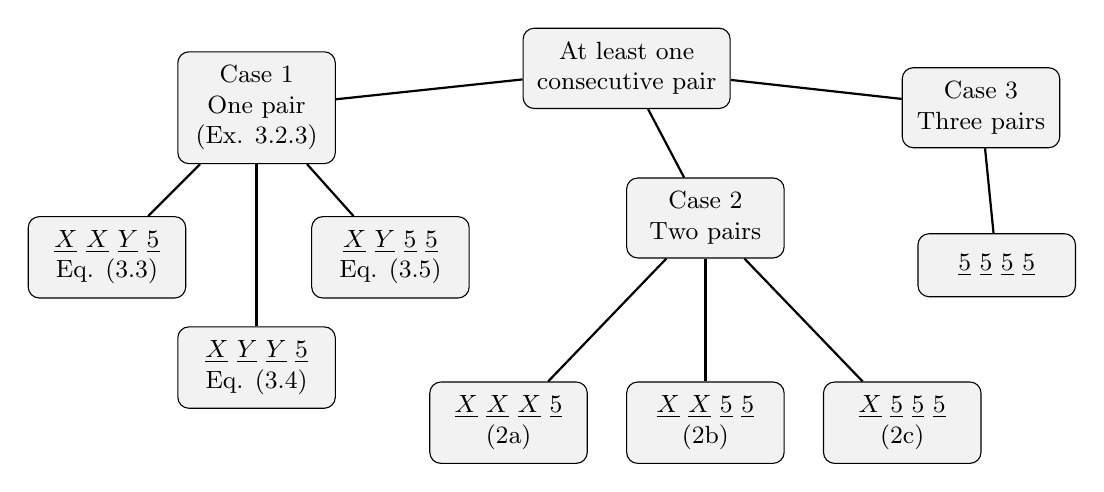
\begin{tikzpicture}[
  every node/.style={font=\small, align=center},
  box/.style={draw, rounded corners, fill=gray!10, inner sep=5pt, minimum width=2cm, minimum height=0.8cm},
  line/.style={draw, thick}
]

% Root node
\node[box] (root) at (0, 0) {At least one\\consecutive pair};

% Level 1 nodes
\node[box] (c1) at (-4.7, -.5) {Case 1\\One pair \\(Ex. 3.2.3)};
\node[box] (c2) at (1, -1.9) {Case 2\\Two pairs};
\node[box] (c3) at (4.5, -0.5) {Case 3\\Three pairs};

% Level 2 nodes - Case 1 children
\node[box] (c1a) at (-6.6, -2.4) {$\underline{X}~\underline{X}~\underline{Y}~\underline{5}$\\Eq. (3.3)};
\node[box] (c1b) at (-4.7, -3.8) {$\underline{X}~\underline{Y}~\underline{Y}~\underline{5}$\\Eq. (3.4)};
\node[box] (c1c) at (-3, -2.4) {$\underline{X}~\underline{Y}~\underline{5}~\underline{5}$\\Eq. (3.5)};

% Level 2 nodes - Case 2 children
\node[box] (c2a) at (-1.5, -4.5) {$\underline{X}~\underline{X}~\underline{X}~\underline{5}$\\(2a)};
\node[box] (c2b) at (1, -4.5) {$\underline{X}~\underline{X}~\underline{5}~\underline{5}$\\(2b)};
\node[box] (c2c) at (3.5, -4.5) {$\underline{X}~\underline{5}~\underline{5}~\underline{5}$\\(2c)};

% Level 2 nodes - Case 3 child
\node[box] (c3a) at (4.7, -2.5) {$\underline{5}~\underline{5}~\underline{5}~\underline{5}$};

% Lines from root to level 1
\draw[line] (root) -- (c1);
\draw[line] (root) -- (c2);
\draw[line] (root) -- (c3);

% Lines from Case 1 to its children
\draw[line] (c1) -- (c1a);
\draw[line] (c1) -- (c1b);
\draw[line] (c1) -- (c1c);

% Lines from Case 2 to its children
\draw[line] (c2) -- (c2a);
\draw[line] (c2) -- (c2b);
\draw[line] (c2) -- (c2c);

% Lines from Case 3 to its child
\draw[line] (c3) -- (c3a);

\end{tikzpicture}
}
\end{center}

Such a diagram is extremely useful for bookkeeping and making sure all cases are accounted for and mutually exclusive.

Breaking up the problem into cases similar to this is an invaluable method. Later, in Chapter 7, we will discuss methods of counting such as double counting and the principle of inclusion-exclusion to reduce the number of cases and find a better approach to problems involving cases. However, for small problem such as these where the cases are relatively easy to compute, there is no harm in breaking the problem up into many cases. 

In fact, there is a famous example of the proof of the Four Color Theorem, the details of which are not important for us right now. What is fascinating, however, is the methods of proof; researchers Kenneth Appel and Wolfgang Haken split the problem into over 1,400 cases, and verified each separately with the help of a computer! The moral of the story is: do not be afraid of "messy" casework!












\section{Direct Counterexample}
The counterexample is another powerful method of proofs. For now, we focus on the simplest method of counterexample, via direct proof. We will later use counterexample in existence proofs, combined with proof by contradiction for a very strong method of proofs. 

The counterexample essentially proves a statement false. Consider the following statement (albeit very simple) as an example.
\begin{example}
Prove that for all integers $x \leq 0$, $\sqrt{x}$ is an imaginary number.
\end{example}
\begin{proof}
This is false. Consider the counterexample $x=0$. $\sqrt{0}=0 \in\mathbb{R}$ and is not an imaginary number. Therefore the statement is not true. 
\end{proof}

The counterexample is usually a method of disproving a statement (which, at-least in research mathematics, is as exciting as a discovery as proving it). The condition says that the statement must be true for all $x \geq 0$. Since $0 \geq 0$ is true, we test $x = 0$. We found that the statement does not hold for $x=0$, and so it does not hold for all $x \geq 0$; it only holds for some. The power comes in that instead of analyzing all numbers greater than or equal to zero, we simply analyze one case which we believe to be a counterexample and thus prove the statement false. Note that to disprove a "for all" statement, we only need there to exist one counterexample (there may be more) to have a definitive conclusion. This seemingly simple technique can be used across various problems. Consider the next example.

\begin{example}
Prove the following statement false. 
\[
a^2 > b^2 \implies a > b
\]
\end{example}
\begin{proof}
Consider the counterexample where $a = -2$ and $b = 1$. $a^2 = 4 > 1 = 1^2$ shows the first condition to be true. However,
\[
-2 \ngeq 1
\]
and thus the statement is not true. The truth of $a^2 > b^2$ does not imply the truth of $a > b$. The statement is true if and only if $a, b \geq 0$.
\end{proof}

\begin{example}
Let $\mathbb{P}\subset \mathbb{N}$ be the set of positive prime integers. Prove or disprove the following statement:
\[
p \in \mathbb{P} \implies 2^p - 1 \in \mathbb{P}
\]
\end{example}
\begin{proof}
We embark on a search for a counterexample.
\[
p = 2 \implies 2^2 - 1 = 3 \in \mathbb{P}
\]
\[
p = 3 \implies 2^3 - 1 = 7 \in \mathbb{P}
\]
\[
p = 5 \implies 2^5 - 1 = 31 \in \mathbb{P}
\]
\[
p = 7 \implies 2^7 - 1 = 127 \in \mathbb{P}
\]
\[
p = 11 \implies 2^{11} - 1 = 2047=23 \times 89, ~~ 2047 \notin \mathbb{P}
\]
Which is a counterexample to the claim. Therefore, the statement is false.
\end{proof}

An important remark is that it is hard to be motivated to search for a counterexample. In this case, searching for a counterexample required us to simply bash through numbers until we found one, which itself is not guaranteed. In areas of research, such boring and menial tasks are often left to computer programs. For example, the famous Goldbach conjecture (every even number can be written as the sum of two primes) has been checked for numbers up until  around 4 quintillion, which is 
\[
4,000,000,000,000,000,000
\]
It is a blessing that humans do not have to manually do such tasks!

While the examples shown were relatively simple, you are now equipped with a basic knowledge of direct counterexample. While this is relatively rare in competition mathematics (manually checking rarely leads to nontrivial counterexamples), it is usually a powerful method when it is properly used. Further, when we study existence and revisit this topic, the counterexample will become a very important concept. 

Further note that not all examples are obviously true (or false) or as simple as the ones shown. One of my favorite "counterexamples" to that notion is Euler's sum of powers conjecture. It states that for an integer ($n \geq 3$), the equation
\[
x_1^n + x_2^n + \cdots + x_k^n = z^n
\]
\noindent has no solution in positive integers when (k < n); that is, at least (n) terms are required to express an (n)th power as a sum of (n)th powers. This conjecture can be viewed as a generalization of Fermat's Last Theorem, which states that no such solutions exist when ($k = 2$) and ($n \geq 3$). However, Euler’s conjecture is false. In 1966, Lander, Parkin, and Selfridge found a counterexample for ($n = 4$):
\[
95800^4 + 217519^4 + 414560^4 = 422481^4 
\]
\[
= 31858749840007945920321
\]

This demonstrates that even statements which appear to extend well-established patterns may fail in unexpected ways! Finding a counterexample is the key here. 


\section{A Note On Thoroughness}
Thus far, we have been quite thorough with our theorems, proving nearly everything from the ground up. If you were to take an Analysis class or something similar (especially in a logic class), you would usually be required to be as thorough, if not more thorough, as we have been in the preceding sections. However, for most competition cases, we do not need to do so. If a statement is trivial in that those with a basic math knowledge understand why it is true (i.e. in the case of $a + b$ is even for odd $a$ and $b$, or that $q$ is even if $q^2$ is even), we do not need to prove it once again. A proof is a demonstration by which we prove a further theorem, and if some statement has already been proved by others, there is no need to reinvent the wheel, so to speak. Similar to computer science, where programmers usually re-use existing libraries, APIs, and infrastructure such as PyTorch or Google Cloud to build apps instead of writing their own code from scratch to interface with the CPU, GPU, etc. However, be careful in that oftentimes, you will need to state theorems by name. For example, we would want to state that we consider two triangles similar by Side-Angle-Side (SAS) similarity instead of claiming they are similar by similarity rules. However, we would not need to reinvent the wheel in proving the Pythagorean theorem, or that $\sqrt{2}$ is irrational, or something of the sort. 

The end goal of constructing a proof, in nearly all cases, is to convey to the reader the methodology by which you have logically come to a conclusion about a certain statement. Thus, as a writer, it is up to you to appropriately assess the thoroughness of your proofs. For competitions, your end goal is to showcase your knowledge and ability to apply knowledge and logic, and thus you may want to exhibit specific information you have used to solve a problem, such as Homothecy or Wilson's theorem. The grader may not find it useful or necessary to understand your knowledge about basic knowledge such as the Pythagorean Theorem or basic facts with numbers. While I have tried my best to explain the thoroughness needed in such a competitive scenario, it may help to view others' solutions to competition problems. With regards to thus, I implore you to search online for IMO shortlist solutions, or USA(J)MO solutions (which can be found on AoPS), or others' solutions on YouTube. 

Further, the standard differ slightly in formal research, or an otherwise academic setting. In classes, it is important to ask the instructor or professor for any questions related to the thoroughness of proofs. In research settings, you may gain a better idea of proofs and the depth by searching for research online, through websites such as arXiv or ResearchGate\footnote{Take caution! Some of the proofs presented here are quite dense and technical and might not help your understanding of mathematical proofs. Thus, browse with caution!}. 


\section{Problems}

\begin{problem}
Prove that $n^2 + n$ is always even by direct proof ONLY. (without casework) \hints{H1}
\end{problem}

\begin{problem}
Prove that for positive integers, 
$
(b \mid a \text{ and } a \mid b) \implies a = b
$
\end{problem}

\begin{problem}
    Find all $x \in \mathbb{R}$ such that 
    \[
    |x+2| + |x-1| \leq 4
    \]
    \hints{H4}
\end{problem}

\begin{problem}
Prove that for any prime number $p$,
$
p \mid a \iff p \mid a^2
$ \hints{H79} \hfill $\star$
\end{problem}

\begin{problem}
Prove or disprove the following statement: for all integers $a$ and $b$,
\[
(a + b)^2 = a^2 + b^2
\]
If the statement is false, find and prove the precise condition on $a$ and $b$ 
under which equality holds.
\end{problem}

\begin{problem}
Find, with proof, all integers $x$ satisfying
\[
x^2 + 3x \equiv 0 \pmod{5}
\]
\end{problem}

\begin{problem}
Let $a, b > 0$. Prove that 
\[
a + \frac{1}{a} \geq 2
\]
When does equality hold?
\end{problem}

\begin{problem}
Let $a, b, c > 0$ with $a + b + c = 1$. Prove that
\[
ab + bc + ca \leq \frac{1}{3}
\]
\hints{H34, H82}\hfill $\star$
\end{problem}

\begin{problem}
Let $P(x) = x^3 + 2x^2 - 5x + 1$. Prove that 
\[
7 \mid P(a) - P(b)
\]
for all integers $a \equiv b \pmod{7}$. \hints{H5}
\end{problem}

\begin{problem}
Let $r_1, r_2, r_3$ be the roots of the polynomial 
\[
f(x) = 2x^3 - 3x^2 + x - 5
\]
Find the value of each of the following without solving for the roots explicitly.
\begin{enumerate}[label=(\alph*)]
    \item $r_1 + r_2 + r_3$
    \item $r_1r_2 + r_1r_3 + r_2r_3$
    \item $r_1^2 + r_2^2 + r_3^2$
\end{enumerate}
\hints{H45, H72}
\end{problem}

\begin{problem}
The ''harmonic mean'' of a collection of numbers is the reciprocal of the arithmetic mean of the reciprocals of the numbers in the collection. For example, the harmonic mean of $4,4,$ and $5$ is
\[\frac{1}{\frac{1}{3}(\frac{1}{4}+\frac{1}{4}+\frac{1}{5})}=\frac{30}{7}.\]
Find, with proof, the harmonic mean of all the real roots of the $4050$th degree polynomial
\[\prod_{k=1}^{2025} (kx^2-4x-3)=(x^2-4x-3)(2x^2-4x-3)...(2025x^2-4x-3)?\]
\hints{H37, H85, H56}\hfill \textit{Adapted from 2025 AMC 12A \#12  }$\star$
\end{problem}

\begin{problem}
Find, with proof, all positive integers $n$ for which $2^n + 12^n + 2011^n$ is a perfect square. 

\hints{H52, H62, H76}\hfill \textit{2011 USAJMO \#1  }$\star$
\end{problem}


